\chapter{Fundamentals}

\section{What is a graph?}%
\label{sec:1.1whatisagraph}

A graph is a pair consisting of vertices and edges. It is usually denoted $G = (V,E)$.

\begin{figure}[ht]
	\centering
	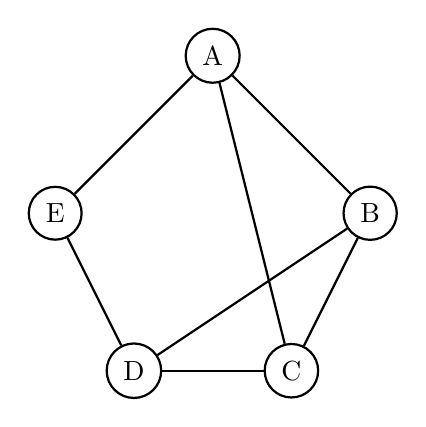
\begin{tikzpicture}[node distance={30mm}, thick, main/.style = {draw, circle}]

		\node[main] (A) at (0,0) {A};
		\node[main] (B) at (2,-2) {B};
		\node[main] (C) at (1,-4) {C};
		\node[main] (D) at (-1,-4) {D};
		\node[main] (E) at (-2,-2) {E};

		\draw (A) -- (B);
		\draw (B) -- (C);
		\draw (C) -- (D);
		\draw (D) -- (E);
		\draw (E) -- (A);
		\draw (A) -- (C);
		\draw (B) -- (D);
	\end{tikzpicture}
	\caption{\label{fig:graph1} A graph $G = (V,E)$}
\end{figure}

The graph seen in Figure~\ref{fig:graph1} features set of vertices $V = \{A, B, C, D, E\}$ and edges $E = \{AB, BC, CD, DE, EA, BD, AC\}$.

We say that an edge has \textit{endpoints}, which it \textit{connects}. Therefore, the edge $AB$ has endpoints $A$ and $B$.

It is important to remember that the visual representation seen of the graph in Figure~\ref{fig:graph1} is only a representation. The graph itself is just the set of vertices and edges connecting the vertices. Therefore, the graph can be represented in many ways, even graphically.

An edge can also be a \textbf{loop}. A loop is an edge that goes from a vertex and goes back to the same vertex without having any vertices in between. An example can be seen in Figure~\ref{fig:loop}.

\begin{figure}[ht]
	\centering
	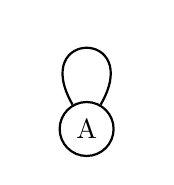
\begin{tikzpicture}[node distance={30mm}, thick, main/.style = {draw, circle}]

		\node[main] (A) at (0,0) {A};

		\draw (A) to[out=60, in=120, looseness=8] (A);
	\end{tikzpicture}
	\caption{\label{fig:loop} A loop.}
\end{figure}

Furthermore, a graph can contain \textbf{multiple edges} (also called \textbf{parallel edges}). This allows to edges to have the same pair of endpoints. And example of this can be seen in Figure~\ref{fig:parallel-edges}.

\begin{figure}[ht]
	\centering
	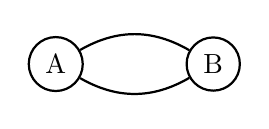
\begin{tikzpicture}[node distance={30mm}, thick, main/.style = {draw, circle}]

		\node[main] (A) at (0,0) {A};
		\node[main] (B) at (2,0) {B};

		\draw (A) to[bend left] (B);
		\draw (A) to[bend right] (B);
	\end{tikzpicture}
	\caption{\label{fig:parallel-edges} Parallel Edges.}
\end{figure}

\begin{definition}[Simple Graph]
	A \textbf{simple graph} is a graph without loops or parallel edges. Thus $\forall e \in E(G)$ $e$ is unique, and its endpoints cannot be the same.
\end{definition}

Two vertices connected by an edge are said to be \textbf{adjacent}. Given two adjacent vertices $A$ and $B$ this can be written $A \leftrightarrow B$. Additionally, we say that $A$ is a neighbour of $B$, and $B$ is a neighbour of $A$. The edge $AB$ is \textit{incident} to the vertex $A$ and $B$.

To introduce the concept of \textit{complement graphs} we will come up with an example of modeling graphs.

\begin{example}
	Consider six people, $a, b, c, d, e, f$. Amongst these people, each two persons are either friends, or strangers. We can turn this into a graph, calling it the friendship-graph. For each person $a$ we have a vertex, and for each friendship, we have an edge between the vertices.


	\begin{center}

		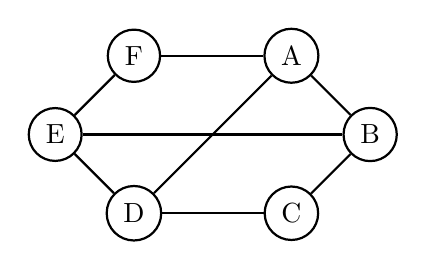
\begin{tikzpicture}[node distance={30mm}, thick, main/.style = {draw, circle}]

			\node[main] (F) at (-1,0) {F};
			\node[main] (A) at (1,0) {A};
			\node[main] (B) at (2,-1) {B};
			\node[main] (C) at (1,-2) {C};
			\node[main] (D) at (-1,-2) {D};
			\node[main] (E) at (-2,-1) {E};

			\draw (A) -- (B);
			\draw (B) -- (C);
			\draw (C) -- (D);
			\draw (D) -- (E);
			\draw (E) -- (F);
			\draw (F) -- (A);
			\draw (E) -- (B);
			\draw (D) -- (A);
		\end{tikzpicture}
	\end{center}

	This graph shows the friendships between the six people. However, it also implicitly shows how many are strangers, namely those who do not have an edge between them. If we turn this into a graph, where there is an edge between all those vertices where there was not an edge before, we get the \textit{complement}  of this graph, written $\overline{G}$.
	\begin{center}

		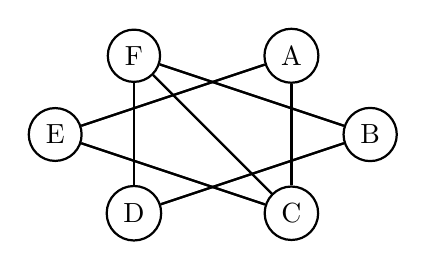
\begin{tikzpicture}[node distance={30mm}, thick, main/.style = {draw, circle}]

			\node[main] (F) at (-1,0) {F};
			\node[main] (A) at (1,0) {A};
			\node[main] (B) at (2,-1) {B};
			\node[main] (C) at (1,-2) {C};
			\node[main] (D) at (-1,-2) {D};
			\node[main] (E) at (-2,-1) {E};

			\draw (F) -- (B);
			\draw (F) -- (C);
			\draw (F) -- (D);
			\draw (A) -- (E);
			\draw (A) -- (C);
			\draw (B) -- (F);
			\draw (B) -- (D);
			\draw (C) -- (A);
			\draw (C) -- (F);
			\draw (C) -- (E);
			\draw (D) -- (F);
			\draw (D) -- (B);
			\draw (E) -- (A);
			\draw (E) -- (C);
		\end{tikzpicture}
	\end{center}

	Thus we can make the connection that $e \in E(G) \iff e \notin E(\overline{G})$.
\end{example}

A \textbf{clique} in a graph $G$ is a set of pairwise adjacent vertices.

\begin{figure}[ht]
	\centering
	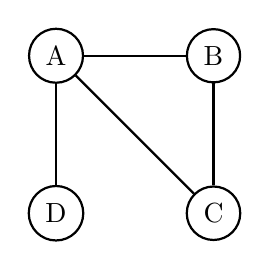
\begin{tikzpicture}[node distance={30mm}, thick, main/.style = {draw, circle}]

		\node[main] (A) at (0,0) {A};
		\node[main] (B) at (2,0) {B};
		\node[main] (C) at (2,-2) {C};
		\node[main] (D) at (0,-2) {D};

		\draw (A) to (B);
		\draw (B) to (C);
		\draw (C) to (A);
		\draw (D) to (A);
	\end{tikzpicture}
	\caption{\label{fig:clique} A graph with a clique $\{A, B, C\}$.}
\end{figure}

In Figure~\ref{fig:clique} is a representation of a graph with a clique $\{A, B, C\}$. The $D$ however, is not part of the graph, as it is not connected to all other vertices.

On the other end is the \textbf{independent} (or \textbf{stable}) set, which is a set of pairwise nonadjacent vertices. In Figure~\ref{fig:clique} an example as $\{D, C\}$ as they have no edges in common.


A \textbf{bipartite} graph is a graph which can be partitioned into two (possibly empty) disjoint independent sets.


\begin{figure}[ht]
	\centering
	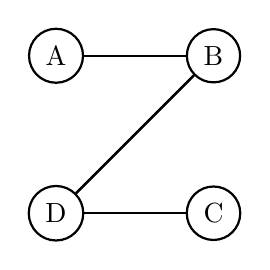
\begin{tikzpicture}[node distance={30mm}, thick, main/.style = {draw, circle}]

		\node[main] (A) at (0,0) {A};
		\node[main] (B) at (2,0) {B};
		\node[main] (C) at (2,-2) {C};
		\node[main] (D) at (0,-2) {D};

		\draw (A) to (B);
		\draw (B) to (D);
		\draw (D) to (B);
		\draw (C) to (D);
	\end{tikzpicture}
	\caption{\label{fig:bipartite} A bipartite graph.}
\end{figure}

In Figure~\ref{fig:bipartite} we see a graph which can be partitioned into two sets $X = \{A, D\}$ and $Y = \{B, C\}$ who have no edges in common. We can generalize this to be more than two partitions, in that case we call it a $k$-partite graph.

With the notion of $k$-partite graphs we can introduce the concept of \textbf{graph colouring}. Given a graph $G = (V,E)$, how many colors do we need, such that each vertex has a different color than its neighbours? For a bipartite graph, the answer is 2. In general, for a $k$-partite graph, the answer is $k$.


Moving on to the notion of \textit{paths} and \textit{cycles}. A \textbf{path} is a sequence of distinct adjacent vertices. A \textbf{cycle} is identical to a path, except it must begin and end with the same vertex. Examples can be seen in Figures~\ref{fig:cycle} and~\ref{fig:path}.

\begin{figure}[ht]
	\centering
	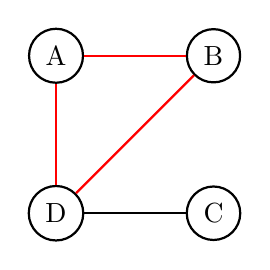
\begin{tikzpicture}[node distance={30mm}, thick, main/.style = {draw, circle}]

		\node[main] (A) at (0,0) {A};
		\node[main] (B) at (2,0) {B};
		\node[main] (C) at (2,-2) {C};
		\node[main] (D) at (0,-2) {D};

		\draw[red] (A) to (B);
		\draw[red] (B) to (D);
		\draw[red] (D) to (A);
		\draw (C) to (D);
	\end{tikzpicture}
	\caption{\label{fig:cycle} A cycle $\{A, B, D\}$.}
\end{figure}
\begin{figure}[ht]
	\centering
	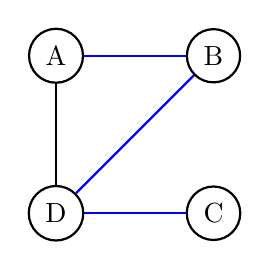
\begin{tikzpicture}[node distance={30mm}, thick, main/.style = {draw, circle}]

		\node[main] (A) at (0,0) {A};
		\node[main] (B) at (2,0) {B};
		\node[main] (C) at (2,-2) {C};
		\node[main] (D) at (0,-2) {D};

		\draw[blue] (A) to (B);
		\draw[blue] (B) to (D);
		\draw (D) to (A);
		\draw[blue] (C) to (D);
	\end{tikzpicture}
	\caption{\label{fig:path} A path $\{A, B, D, C\}$.}
\end{figure}

A \textbf{subgraph} is part of another graph. We say that $H$ is a subgraph of $G$ if $V(H) \subseteq V(G)$ and $E(H) \subseteq E(G)$. Furthermore, we say that $G$ \textbf{contains} $H$. As paths and cycles are both subgraphs, we can say that a graph $G$ can \textit{contain} a specific path or cycle.

So far we have only looked at visual representations of graphs in the form of circles as vertices and lines as edges. You can also represent graphs as matrices. Given a graph $G = (V,E)$ where $V = \{A, B, C, D\}$ and $E = \{E_{1}, E_{2}, E_{3}, E_{4}, E_{5}\}$ where $E_{1} = ab, E_{2} = bc, E_{3} = bc, E_{4} = ac$ and $E_{5} = cd$ we can represent these as an \textit{Adjacency Matrix} and an \textit{Incidence Matrix}. An adjacency matrix is a matrix where $A_{i,j}$ contains the number of edges between $i$ and $j$. This also means that the adjacency matrix is symmetric. In the \textit{incidence matrix} $M_{i,j}$ contains a $1$ if $j$ is an edge which is incident to $j$. This means that the incidence matrix' size is determined by the number of edges \textit{and} vertices, while the adjacency matrix' size is determined solely by the number of vertices.

% First matrix (Adjacency Matrix)
The adjacency matrix:
\[
	\begin{array}{c|cccc}
		  & a & b & c & d \\
		\hline
		a & 0 & 1 & 1 & 0 \\
		b & 1 & 0 & 2 & 0 \\
		c & 1 & 2 & 0 & 1 \\
		d & 0 & 0 & 1 & 0 \\
	\end{array}
\]

\hspace{1cm} % Horizontal space between the two matrices

The incidence matrix:
% Second matrix (Incidence Matrix)
\[
	\begin{array}{c|ccccc}
		  & e_1 & e_2 & e_3 & e_4 & e_5 \\
		\hline
		a & 1   & 0   & 0   & 1   & 0   \\
		b & 1   & 1   & 1   & 0   & 0   \\
		c & 0   & 1   & 1   & 1   & 1   \\
		d & 0   & 0   & 0   & 0   & 1   \\
	\end{array}
\]

Now we turn to the question of \textbf{isomorphism}. Given two graphs $G$ and $H$, is there a function $f : V(G) \rightarrow V(H)$ that maps such that $uv \in E(G) \iff f(u)f(v) \in  E(H)$. If such a function exists, we say that $G$ is \textbf{isomorphic} to $H$. We write this $G \cong H$.

We define the \textit{isomorphism class} to be an equivalence class of graphs under the isomorphism relation. I.e., all graphs that are isomorphic to each other form an isomorphism class.

Given a graph with $n$ vertices, how many graphs are possible? I.e., how many ways can we arrange the edges? Given a pair of vertices, there are two options: either an edge connects them, or there is no edge to connect them. Thus there are $2^{\binom{n}{2}}$ possible graphs on $n$ vertices. The question of how many isomorphism classes there are on $n$ vertices is not easy to answer.

Some other classes of graphs are:
\begin{itemize}
	\item $P_{n}$: A path with $n$ vertices.
	\item $C_{n}$: A cycle with $n$ vertices.
	\item $K_{n}$: A complete graph with $n$ vertices.
\end{itemize}
In a complete graph, all vertices are pairwise adjacent, meaning there is an edge between all vertices. We denote the complete graph $K_{n}$, and the \textbf{complete bipartite graph} $K_{r,s}$ where $r$ is the number of vertices in one set and $s$ the number of vertices in the other. Then for each $v \in R$, there is an edge to all $v \in S$, and the other way around. However, there is no edge between the vertices in respectively $R$ and $S$.

A special graph, the Petersen graph, is probably the most famous graph in all of graph theory. The graph is the result of  the following statement: $(ij)$ and $(kl)$ are adjacent if $\{i,j\} \cap \{k,l\} = \emptyset$.

A graph is said to be \textbf{self-complementary} if it is isomorphic to its complement. Some examples are $P_{4}$ and $C_{5}$.

The \textbf{decomposition} of a graph is a list of subgraphs such that every edge appears in exactly one subgraph in the list.

The \textbf{girth} of a graph is the length of its shortest cycle.

An automorphism of $G$ is an isomorphism from $G$ to itself. A graph is said to be \textbf{vertex-transitive} if for every pair $u, v \in V(G)$ there exists an automorphism that maps $u$ to $v$.

\section{Paths, Cycles and Trails}%
\label{sec:label}

As we have already talked about briefly, paths are sequences of vertices and edges $v_{0}e_{1}v_{1}\ldots e_{k}v_{k}$. Trails and paths are the same. However, we distinguish between these as such:
\begin{itemize}
	\item \textbf{Walk}: No constraints.
	\item \textbf{Trail}: All edges must be distinct.
	\item \textbf{Path}: All vertices must be distinct (and by extension edges).
\end{itemize}

We write $(u,v)$-(walk,path,trail) in order to specify a (walk,path,trail) which starts at vertex $u$ and ends at vertex $v$.

\begin{lemma}
	Every $(u,v)$-walk contains a $(u,v)$-path.
\end{lemma}

\begin{proof}
	We prove this by induction on the number of edges, $m$. The walk itself we call $W$.\\
	\noindent
	\textbf{Base Case $m = 0$}: $W$ is a $(u,v)$-path with 1 vertex.\\
	\noindent
	\textbf{Inductive Step}: Assume true for all smaller $m$.\\
	\noindent
	If no vertex in walk $W$ repeats, then $W$ is a $(u,v)$-path. If a vertex repeats, then we can write the walk as $v_{0}v_{1}v_{2} \cdots v_{i} \cdots v_{j}v_{j+1} \cdots v_{k}$ where the path has length $k$. In this case, there must be an $i$ and $j$ such that $v_{i} = v_{j}$. Thus, we can ignore the part between, $v_{i}v_{i+1} \cdots v_{j-2}v_{j-1}$, and have a resulting $(u,v)$-path.
\end{proof}

We say that a graph $G$ is connected, if $\forall u,v \in V(G)$ there is a $(u,v)$-path. The connected \textbf{components} of $G$ are the maximal connected components of $G$.

The \textbf{order} of the graph is the number of vertices. The \textbf{size} of the graph is the number of edges.
\begin{proposition}
	Every (simple) graph of order $n$ and size $k$ has at least $n-k$ components.
\end{proposition}
\begin{proof}
	We prove by induction on the number of edges $m$.\\
	\noindent
	\textbf{Base Case} $m = 0$: A graph with $n$ vertices and $0$ edges has $n - k = n - 0 = n$ components.\\
	\noindent
	\textbf{Inductive Step}: Assume for smaller $m$.\\
	\noindent
	Given a graph with $n$ vertices and $k$ edges, if we remove one edge, we can at most add one new component.
\end{proof}

A vertex $v \in V(G)$ is a \textit{cut-vertex} if deleting $v$ increases the number of components. Similarly, an edge $e \in E(G)$ is \textit{cut-edge} if deleting it increases the numbre of components.

\begin{theorem}
	An edge is a cut-edge if and only if it belongs to no cycle.
\end{theorem}
\begin{proof}
	$\Rightarrow$\\
	\noindent
	Assume that the edge is not a cut edge, if it belongs to no cycle. Thus, removing it would not create a new component. However, it would create a new component, as when there is no cycle it must be split into two. This is a contradiction.\\
	\noindent
	$\Leftarrow$\\
	\noindent
	TONCAS.
\end{proof}

\begin{theorem}[König 1936]
	A graph is bipartite if and only if it has no odd cycle.
\end{theorem}

\begin{proof}
	Let $G$ be a bipartite graph with partite sets $A$ and $B$.\\\\
	\noindent
	$\Rightarrow$\\
	\noindent
	Starting a walk in $A$, the walk will alternate between the partite sets $A$ and $B$ between each edge. Thus, when it returns it will have an even number of edges. Therefore, the cycle will be even.\\
	\noindent
	$\Leftarrow$\\
	\noindent
	We prove this for each component of $G$.
	Let $C$ be a component of $G$ and let $x \in V(C)$. For each $y \in V(C)$ let $f(y)$ be the distance from $x$ to $y$. This distance is the shortest distance, and thus the length of the shortest $(x,y)$-path.

	Let $X = \{u \mid f(u) \text{ is even}\}$ and $Y= \{u \mid f(u) \text{ is odd}\}$. We will show that $X$ and $Y$ are independent, and thus $C$ is bipartite.

	For the sake of contradiction, assume that there is an edge $v_{1}v_{2} \in E(C)$ in $Y$ (or $X$). There exists  a $(x,v_{i})$-path $P_{i}$ of length $f(v_{i})$ for $i = 1,2$. Let $z \in V(P_{1}) \cap V(P_2)$ be chosen such that $f(z)$ is maximum. This would mean that $z$ is the last common vertex, as they diverge at some point (last common as we use intersection).

	Let $P_{i}'$ be the $(z,v_{i})$-subpath of $P_{i}$, for $i = 1,2$. $|E(P_{i}')| = f(v_{i}) - f(z)$ for $i = 1,2$. That is, the number of edges in $P_{i}'$ is equal to $f(v_{i}) - f(z)$ where $f(v_{i})$ is the length from $x$ to $v_{1}$ and $v_{2}$. Thus $P_{i}'$ is simply the subgraph containing the paths from the vertex before the paths diverge until the end.

	Consider the cycle $R$. We define $R$ to be the union of the edges of the two paths $P_{i}'$ along with the edge $\{v_{1}v_{2}\}$.  Thus $E(R) = E(P_{1}') \cup E(P_{2}') \cup \{v_{1}v_{2}\}$. $|E(R)| = f(v_{1}) - f(z) + f(v_{2}) - f(z) + 1 = f(v_{1}) + f(v_{2}) - 2f(z) + 1$. We get the $+1$ from the edge $\{v_{1}v_{2}\}$. However, we encounter a contradiction here, $E(R)$ is odd! Thus this cannot be possible, and every graph without an odd cycle is bipartite.
\end{proof}

An \textbf{Eulerian Circuit} is a \textit{closed trail} (a trail which starts and ends with the same vertex) which traverses all edges exactly once. A graph has an Eulerian Circuit (and is said to be Eulerian itself) if and only if it is connected and every vertex has an even degree.

\begin{proposition}
	Every graph containing at least one (nonloop) edge has at least two vertices that are not cut-vertices.
\end{proposition}
\begin{proof}
	If $u$ is an endpoint of a maximal path $P$ in $G$, then the neighbours of $u$ lie on $P$. Since $P-u$ is connected in $G-u$, the neighbours of $u$ belong to a single component of $G-u$ and $u$ is not a cut vertex.
\end{proof}

\section{Vertex Degrees and Counting}%
\label{sec:1.3}


The \textbf{degree} $d_{G}(v)$ or $d(v)$ is the number of edges incident to $v$. Remark that a loop is incident twice, and therefore adds two to the degree count. We define $\delta(G)$ to be the vertex of minimum degree in a graph $G$. Similarly, $\Delta(G)$ is the vertex with maximum degree in a graph $G$.

A graph is said to be $k$-regular, if all vertices have degree $k$. Therefore, if $\delta(G) = k = \Delta(G)$ then $G$ is $k$-regular.

\begin{theorem}[Degree-Sum-Formula]
	If $G$ is a graph, then
	\begin{equation}
		\sum_{v \in V(G)} d(v) = 2|E(G)|
	\end{equation}
\end{theorem}
\begin{proof}
	Summing the degrees counts each edge twice, since each edge has two endpoints, and we count each endpoint once.
\end{proof}

We can now answer the following question: ``What is the average degree of a graph of order $n$ and size $m$?''.

\begin{equation}
	\frac{\sum_{u \in V(G)} d(u)}{n} = \frac{2|E(G)|}{n} = \frac{2m}{n}
\end{equation}

We now present some corollaries:

\begin{corollary}
	In any graph $G$:
	\begin{equation}
		\delta(G) \le \frac{2|E(G)|}{n} \le \Delta(G)
	\end{equation}
\end{corollary}

\begin{corollary}
	Every even graph has an even number of odd degree vertices. No graph of odd order is regular with an odd degree.
\end{corollary}

This corollary comes from the fact that graphs without these properties would be impossible to produce.

\begin{corollary}
	A $k$-regular graph with $n$ vertices has $\frac{nk}{2}$ edges.
\end{corollary}

This comes from the fact that every vertex has degree $k$, and as there are $n$ vertices, we get $nk$ edges counted using the degree-sum formula. We divide this by $2$ to remove the double-counted edges.

We now introduce a new family of graphs: \textit{Hypercubes}. A $k$-dimensional hypercube $Q_{k}$ has vertices which are bit-strings of length $k$. Given a function $f(a,b)$ which takes two bit strings of the same length, and returns $1$ if the bit strings differ by \textit{exactly} one bit, and zero otherwise. We can now determine how the edges in the hypercube $Q_{k}$ is constructed:

\begin{equation}
	f(u,v) = \begin{cases}
		1 & uv \text{ is an edge in } G     \\
		0 & uv \text{ is not an edge in } G
	\end{cases}
\end{equation}

To use not-overly-complicated language: If two vertices differ by one bit, there is an edge between them. If they differ by more than one, there are no edges between them.

There are some interesting properties about hypergraphs. The hypergraph $Q_{k}$ is bipartite, as you can always partition it into two sets if independent vertices. Furthermore $\Delta(Q_{k}) = k = \delta(Q_{k})$. The number of vertices is the number of bitstrings of length $k$, thus $n(Q_{k}) = |V(Q_{k})| = 2^{k}$ and the number of edges $|E(Q_{k})| = \frac{k2^{k}}{2}$ as $2|E(Q_{k})| = \sum_{v \in V(Q_{k})}d(v) = k2^{k}$.

\begin{proposition}
	If $k > 0$ then a $k$-regular bipartite graph has equally many vertices in each partite set.
\end{proposition}

\begin{proof}
	\begin{equation}
		k \cdot |X| = |E(G)| = k \cdot |Y|
	\end{equation}
\end{proof}

\begin{proposition}
	Let $G$ be a simple graph with 	$V(G) = \{v_{1}, \ldots, v_{n}\}$ where $n \ge 3$, then

	\begin{equation}
		|E(G)| = \frac{ \sum_{i=1}^n  |E(G-v_{i})| }{n-2}
	\end{equation}
\end{proposition}
\begin{proof}
	Each edge is counted $n-2$ times in the summation.
\end{proof}

The following conjecture is a very famous open conjecture in Graph Theory:

\begin{conjecture}[Reconstruction Conjecture]
	If $G$ is a simple graph with at least 3 vertices, then $G$ is uniquely determined by the list of its vertex deleted subgraphs.
\end{conjecture}

We will now turn our attention to \textbf{extremal problems}. We give some examples first to show what the concept of extremal problems concerns itself about:
\begin{itemize}
	\item What is the minimum number of edges in a connected graph of order $n$? (Answer: $n-1$)
	\item What is the smallest value $x_{n}$ such that $\delta(G) \ge x_{n}$ implies that $G$ is connected when $n(G) = n$? (Answer: $\frac{n-1}{2}$)
	\item Every loopless graph $G$ has a bipartite subgraph with at least $|E(G)|/2$ edges.
	      \begin{itemize}
		      \item This is an extremal problem, as we can reformulate it like this: ``What is the minimum number of edges we can guarantee in a bipartite subgraph?''.
	      \end{itemize}
	\item What is the maximum number of edges in a graph of order $n$ containing no triangle ($K_{3}$)? (Answer: $\lfloor \frac{n^{2}}{4} \rfloor$).
\end{itemize}

We define the \textbf{neighbourhood} of a vertex $v$ to be the neighbours of $v$. We denote it by $N(v)$. We extend this notation to $N[v] = N(v) \cup \{v\}$.

\begin{proposition}
	If $G$ is a simple graph of order $n$ with $\delta(G) \ge \frac{n-1}{2}$, then $G$ is connected.
\end{proposition}
\begin{proof}
	Choose $u,v \in V(G)$. We show that $u$ and $v$ have a common neighbour if they are not themselves neighbours. Since $G$ is simple, we have $|N(u)|\ge \delta(G) \ge \frac{n-1}{2}$, and similarly for $v$.
	When $u$ and $v$ are not neighbours, we have $|N(u) \cup N(v)| \le n-2$ and $|N[u] \cup N[v]| \le n$.

	Thus we can get $|N(u) \cap N(v)|$:
	\begin{equation}
		|N(u) \cap N(v)| = |N(v)| + |N(u)| - |N(u) \cup N(v)| \ge \frac{n-1}{2} + \frac{n-1}{2} - (n-2) = 1
	\end{equation}
\end{proof}
This is \textbf{best possible} or \textbf{sharp}. This means that we cannot make this argument any stronger, without it being false.


We say that a graph is $H$-free, if it does not contain subgraph $H$.

\begin{theorem}[Mantel]
	The maximum number of edges in a $K_{3}$-free graph of order $n$ is $\lfloor n^{2} /4 \rfloor$.
\end{theorem}
\begin{proof}
	Let $G$ be a graph that is $K_{3}$-free. Let $x \in V(G)$ have maximum degree, say $d(x) = k$. Since $G$ has no triangles, there are no edges among the neighbours of $x$.

	Summing the degrees of $x$ and its nonneighbours counts at least one endpoint of every edge. We sum over $n-k$ vertices as we do not count the $k$ neighbours of $x$, each having degree at most $k$, so $|E(G)| \le (n-k)k$.

	The maximum value of $f(k) = (n-k)k$ is obtained at $k = n/2$ (from $f'(k) = n-2k$).

	Since $k$ is an integer, the maximum value is obtained when $k \in \{ \lceil \frac{n}{2} \rceil, \lfloor \frac{n}{2} \rfloor \}$.

	So, $|E(G)| \le (n-k)k \le \lceil \frac{n}{2} \rceil \cdot \lfloor \frac{n}{2} \rfloor = \lfloor n^{2}/4 \rfloor$.
\end{proof}

The \textbf{degree sequence} of a graph is a list of vertex degrees. Usually we write these in decreasing order. For Figure~\ref{fig:cycle} the degree sequence is \texttt{2221}.

\begin{proposition}
	The nonnegative numbers $d_1 \ldots d_n$ are the degree sequence for some graph if and only if $\sum_{i=1}^n d_{i}$ is even.
\end{proposition}

\begin{proof}
	We will do a constructive proof.
	Assume $\sum_{i=1}^n d_{i}$ is even. For this to be possible, there is an even number of odd values in $d_{1}, \ldots, d_{n}$. Pair these vertices with odd degree up, and add an edge between each pair. Then add $\lfloor  \frac{d_{i}}{2} \rfloor$ loops at each vertex. This will give us a graph with the degree sequence $d_{1}, \ldots, d_{n}$.

	The other direction holds as well, as $\sum_{i=1}^n$ is even, by the degree-sum formula.
\end{proof}

If we look at simple graphs (those who do not allow parallel edges or loops), rather than obtaining a \textit{degree sequence}, we call it a \textbf{graphic sequence}.

\begin{proposition}[Havel-Hakimi]
	Let $n > 1$. An integer list $d$ of size $n$ is graphic if and only if $d'$ is graphic, where $d'$ is obtained from $d$ by deleting the largest element \(\Delta\) and subtracting 1 from the next \(\Delta\) largest elements. The only 1-element graphic sequence is $d_{1} = 0$.
\end{proposition}

Before showing the proof, we will give two examples. One which works, and one which doesn't. If a sequence goes to 0, it works, while if it does not, it does not work.

\begin{example}[An invalid graphic sequence]
	Let's look at the graphic sequence \texttt{5 4 4 2 1 1 1}.

	We remove the first number, 5, and subtract the next 5 numbers. We obtain from this the sequence \texttt{3 3 1 0 0 1}. We remember to sort in decreasing order, \texttt{3 3 1 1 0 0} and repeat the process, thus obtaining \texttt{2 0 0 0 0}. Here comes the problem. we remove 2, and the next two become -1. This is obviously not possible, as there can be no vertex where $d(v) < 0$.
\end{example}

Now for a succesfull example:

\begin{example}[A valid graphic sequence]
	We start with the sequence \texttt{5 3 3 2 2 1}. Continuing from the proposition, we get:
	\begin{enumerate}
		\item \texttt{5 3 3 2 2 1}
		\item \texttt{2 2 1 1 0} - Removing 5 and decreasing the next 5
		\item \texttt{1 1 0 0} - Removing 2 and decreasing the next 2 (sorted)
		\item \texttt{0 0 0} - We remove 1 and decrease the next
		\item \texttt{0 0} - Remove 0
		\item \texttt{0} - Remove 0
	\end{enumerate}
	Thus it is graphic.
\end{example}

\begin{proof}
	Let $d$ be a sequence of $n$ nonnegative integers. Let $d'$ be obtained from the sequence $d$, by deleting the largest number \(\Delta\) and decreasing the next \(\Delta\) numbers.

	The goal of this proof is to show the following:

	\begin{equation*}
		\text{''d is graphic'' } \iff \text{ ''d' is graphic''}
	\end{equation*}

	We start by proving that if $d'$ is graphic, then $d$ is graphic. Let $G'$ be a \textbf{simple graph} with degree sequence $d'$. Add a new vertex, $x$ to $G'$, and connect the vertex to the first \(\Delta\) vertices. Thus we have obtained a simple graph which has degree sequence $d$.
	$\Leftarrow \qed$.\\\\
	\noindent
	We now prove ``if $d$ is graphic, then $d'$ is graphic''. Let $G'$ be a graph with degree sequence $d = (d_{1}, d_{2}, \ldots, d_{n})$. Let $w$ be the vertex where $d(w) = d_{1}$. Let $S$ be a set of $d_{1}$ vertices with degrees $d_{2}, d_{3}, \ldots, d_{d_{1}+1}$ (i.e., the next $d_{1}$ degrees on the graphic sequence). If $N(w) = S$ we are done as $G - w$ has degree sequence $d'$.

	We will now show that, if $N(w) \ne S$, we can increase $|S \cap N(w)|$ until $N(w) = S$. As $|N(w)| = d_{1} = |S|$ there must be a vertex $x \in S \setminus N(w)$, that is, a vertex which has the correct number of degrees, but is not in the neighbourhood of $w$. There must also be $z \in N(w) \setminus S$, i.e., a vertex which is a part of the neighbourhood, but does not have the correct degree. As it does not have the correct degree, it must have a smaller degree than $x$ (as we have chosen the vertex with the highest). Thus there must exist a $y \in N(x) \setminus N(z)$, that is, a vertex which is the neighbour of the vertex which is in the neighbourhood, but not with the correct degree, and a vertex which has the correct degree, but is not in the neighbourhood. (Remark that when I say correct degree, I mean a degree in the degree sequence $d_{2}, \ldots, d_{d_{1}+1}$). If we, from this, delete edges $wz$ and $xy$ and add a new edge $wx$ and $yz$, all degrees stay the same and $|S \cap N(w)|$ is increased.
\end{proof}

\section{Directed Graphs}%
\label{sec:1.4}

A directed graph is simply a graph in which the edges have a direction. These edges are typically called arcs, and the directed graphs are typically called digraphs. In Figure~\ref{fig:digraph} you can see the graph presented in Figure~\ref{fig:graph1}, but with arcs instead of edges.

\begin{figure}[ht]
	\centering
	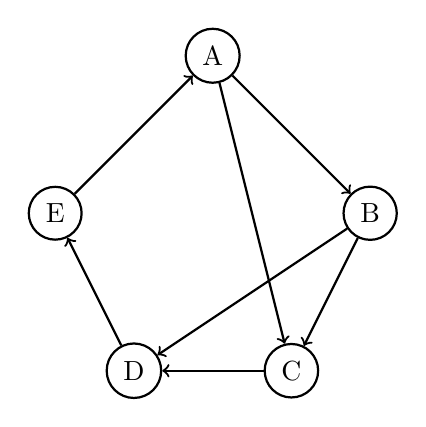
\begin{tikzpicture}[node distance={30mm}, thick, main/.style = {draw, circle}]

		\node[main] (A) at (0,0) {A};
		\node[main] (B) at (2,-2) {B};
		\node[main] (C) at (1,-4) {C};
		\node[main] (D) at (-1,-4) {D};
		\node[main] (E) at (-2,-2) {E};

		\draw[->] (A) -- (B);
		\draw[->] (B) -- (C);
		\draw[->] (C) -- (D);
		\draw[->] (D) -- (E);
		\draw[->] (E) -- (A);
		\draw[->] (A) -- (C);
		\draw[->] (B) -- (D);
	\end{tikzpicture}
	\caption{\label{fig:digraph} A digraph $D = (V,A)$}
\end{figure}

We have some specific terminology for the arcs. The \textbf{head} of the arc $ab$ is $b$, i.e., the vertex it ``points'' to. The \textbf{tail} is $a$, i.e., the vertex it ``emerges from''. As with undirected graphs, paths and cycles still exist, but we now have to follow the direction the arcs point.

The \textbf{underlying graph} of a digraph $D$ is the same graph, but where the arcs are turned into edges. The underlying graph of $D$ from Figure~\ref{fig:digraph} is the graph $G$ found in Figure~\ref{fig:graph1}.

Many definitions are the same for digraphs as they are for non-directed graphs, such as subgraphs, isomorphism etc. Adjacency matrices are slightly different. Rather than the entry $A_{i,j}$ being the number of edges being between vertices $i$ and $j$, there is a $1$ if there is an arc \textbf{from $i$ to $j$}. This means that the adjacency matrix for a digraph is not symmetric. An incidence matrix uses $-1$ and $+1$ to indicate respectively the tail and head of the arc.

Many of the definitions also remain the same, but with some slight tweaks added. For example, connectivity is the same, but with digraphs we distinguish between \textbf{strong} and \textbf{weak} connectivity. For a digraph to be \textbf{strongly connected}, following must hold: $(\forall u,v \in V(D) \mid \exists (u,v) \text{-path})$, i.e., there must be a path for all pairs of vertices. For a digraph to be \textbf{weakly connected}, the underlying graph must be connected. The \textbf{strong components} of a digraph are the maximal strong connected subgraphs.

We define vertex degrees a bit different in digraphs as well. We now distinguish between \textbf{indegrees} $d^{-}(v)$ and \textbf{outdegrees} $d^{+}(v)$. The \textbf{indegree} is the number of arcs pointing to $v$, while the \textbf{outdegree} is the number of arcs emerging from $v$. The degree-sum formula is much like the one for non-directed graphs, however it might be a bit easier to understand.

\begin{theorem}[Degree-sum formula for digraphs]
	\begin{equation*}
		\sum_{v \in V(D)} d^{+}(v) = |E(D)| = \sum_{v \in V(D)} d^{-}(v)
	\end{equation*}
\end{theorem}

\begin{corollary}
	\begin{equation*}
		\sum_{v \in V(D)} d^{+}(v) + \sum_{v \in V(D)} d^{-}(v) = 2|E(D)|
	\end{equation*}
\end{corollary}

\begin{proposition}
	Let $d$ be a list of $n$ pairs. $d = ((d^{+}_{1}, d^{-}_{1}), \ldots, (d^{+}_{n}, d^{-}_{n}))$.

	There exists a digraph $D$ with $V(D) = \{v_{1}, \ldots, v_{n}\}$ such that $d^{+}(v_{i}) = d_{i}^+$ and $d^{-}(v_{i}) = d^{-}_{i}$ if and only if $\sum_{i=1}^n d_{i}^{+} = \sum_{i=1}^n d_{i}^{-}$.
\end{proposition}

\begin{example}
	This also kind of works like a proof.

	Let $d = ((3,1), (2,2), (1,2), (1,2))$.

	\begin{equation*}
		\sum_{i=1}^n d_{i}^{+} = 3 + 2 + 1 + 1 = 7 = 1 + 2 + 2+ 2 = \sum_{i=1}^n d_{i}^{-}
	\end{equation*}

	We now create 7 dots, one for each arc. We first look at $v_{1}$, which has 3 outgoing and one ingoing arc. As it has one ingoing, it can have one loop. Thus the first dot is $(1,-1)$ representing the vertex going from 1 to 1. $v_{2}$ has two incoming edges, and 2 outgoing edges. We can take the remaining edges from $v_{1}$ and put into $v_{2}$, thus going from 1 to into 2, i.e., $(1, -2)$ twice. For $v_{2}$ there are still 2 outgoing arcs. $v_{3}$ has 2 incoming arcs, and therefore both of the arcs from $v_{2}$ can go to $v_{3}$, resulting in the dots $(2, -3)$. $v_{3}$ only has one outgoing edge left, and $v_{4}$ has 2 incoming and 1 outgoing. One of the incoming will come from $v_{3}$ and the other from itself, which will also be an outgoing (i.e., a loop). We end with the following dots:
	\begin{itemize}
		\item $(1, -1)$ - loop on $v_{1}$
		\item $(1, -2)$ and $(1, -2)$ - arcs from $v_{1}$ to $v_{2}$
		\item $(2,-3)$ and $(2,-3)$ - arcs from $v_{2}$ to $v_{3}$
		\item $(3, -4)$ - arc from $v_{3}$ to $v_{4}$
		\item $(4,-4)$ - loop on $v_{4}$
	\end{itemize}
\end{example}

Recall that an \textbf{Eulerian circuit} in an undirected graph  is a closed trail containing all edges. For a digraph it's a closed trail containing all arcs, and it must follow the direction of the arcs.

\begin{theorem}
	A digraph is Eulerian if and only if $\forall v \in V(D) \mid d^{+}(v) = d^{-}(v)$ and the underlying graph has at most one nontrivial component (i.e., a component which contains edges (a trivial component is a single vertex without any edges)).
\end{theorem}

An \textbf{oriented graph} is a graph which is the result of an \textbf{orientation} of an undirected graph. Meaning, for each edge in the undirected graph, we give it a direction. A \textbf{tournament} is an orientation of a complete graph. We call it a tournament, as it can model a round-robin tournament.

A \textbf{king} in a digraph is a vertex $x$ such that there exists a $(x,u)$-path of length at most two for all vertices $u$.

\begin{proposition}[Landau, 1953]
	Every tournament has a king.
\end{proposition}

\begin{proof}
	Let $T$ be any tournament. Recall that a tournament is an orientation of a \textit{complete} graph, not just any graph. Let $x$ be a vertex of maximum outdegree from $T$, and choose an arbitrary $y \in V(T) \setminus \{x\}$.

	\begin{enumerate}
		\item If there exists an arc $xy \in A(T)$, then we have a $(x,y)$-path of length 1
		\item If $xy \notin A(T)$ then $yx \in A(T)$.
	\end{enumerate}
	As $|N^{+}(x)| \ge |N^{+}(y)|$ and $x \in N^{+}(y) \setminus N^{+}(x)$, there must be a $z \in N^{+}(x) \setminus N^{+}(y)$. This implies an $xzy$-path of length 2.
\end{proof}


%%% Local Variables:
%%% mode: latex
%%% TeX-engine: luatex
%%% TeX-command-extra-options: "-shell-escape"
%%% TeX-master: "main"
%%% End:
